% ||||||||||||||||||||||||||||||||||||||||||||||||||||||||||||||||||||
\documentclass{beamer}
\usepackage[utf8]{inputenc}
\usepackage[english]{babel}
\usepackage{amsmath}
\usepackage{setspace}
\usepackage{bm}
\usepackage{graphicx}
\usetheme{CambridgeUS}
\usepackage{stmaryrd}
\usepackage{mathrsfs}
\usepackage[makeroom]{cancel}
\usepackage{amsmath,amsthm,stmaryrd,amssymb,bbm,amsfonts,amstext, graphicx, multicol, array}
\usepackage{mathtools}
\usepackage{color}

\newcommand\vertarrowbox[3][2ex]{%
  \begin{array}[t]{@{}c@{}} #2 \\
  \left\uparrow\vcenter{\hrule height #1}\right.\kern-\nulldelimiterspace\\
  \makebox[0pt]{\scriptsize#3}
  \end{array}%
}

\setbeamercolor{math text}{fg=blue}
\setbeamercolor{math text displayed}{fg=blue}


% ||||||||||||||||||||||||||||||||||||||||||||||||||||||||||||||||||||
% ||||||||||||||||||||||||||||||||||||||||||||||||||||||||||||||||||||
\title{ECON2500 Spring 2025\\ Paper Presentation}
\subtitle{Arellano, Cristina, Mateos-Planas, Xavier and Ríos-Rull, José-Víctor, (2023), Partial Default, Journal of Political Economy, 131, issue 6, p. 1385 - 1439.}
\author{Adrien Foutelet}
\date{\today}
% ||||||||||||||||||||||||||||||||||||||||||||||||||||||||||||||||||||
\AtBeginSection[]{
\begin{frame}
\vfill
\centering
\begin{beamercolorbox}[sep=8pt,center,shadow=true,rounded=true]{title}
\usebeamerfont{title}\insertsectionhead\par%
\end{beamercolorbox}
\vfill
\end{frame}
}
% ||||||||||||||||||||||||||||||||||||||||||||||||||||||||||||||||||||


% ||||||||||||||||||||||||||||||||||||||||||||||||||||||||||||||||||||
% ||||||||||||||||||||||||||||||||||||||||||||||||||||||||||||||||||||
% ||||||||||||||||||||||||||||||||||||||||||||||||||||||||||||||||||||
\begin{document}
% ||||||||||||||||||||||||||||||||||||||||||||||||||||||||||||||||||||
% ||||||||||||||||||||||||||||||||||||||||||||||||||||||||||||||||||||
% ||||||||||||||||||||||||||||||||||||||||||||||||||||||||||||||||||||
%
\maketitle
% ||||||||||||||||||||||||||||||||||||||||||||||||||||||||||||||||||||
% ||||||||||||||||||||||||||||||||||||||||||||||||||||||||||||||||||||
%
\section{Introduction}


\begin{frame}{Motivation}
Financial Times, March 7 2025. "What a Mar-a-Lago accord could look like":
    
\begin{quote}

    \small

    [...] On September 22 1985 [in Plaza Hotel in New York], the US government persuaded Britain, Japan, Germany and France to jointly devalue the dollar, to boost America's industrial competitiveness.

    [...] There has been speculation about a new Plaza Accord — dubbed the "Mar-a-Lago Accord" — to depreciate the US dollar.

    [...] consider a must-read essay from Stephen Miran, Trump's pick for chair of the Council of Economic Advisers.

	[...] while Miran's essay warns that tariffs might initially strengthen the dollar, he thinks Washington can offset this. [...] one idea floating around is that other nations will be “encouraged” to swap holdings of dollars, short-term Treasuries or even gold for long-term or perpetual dollar bonds suitable for repurchase deals at the Federal Reserve.

\end{quote}

Formally, this is default: a sovereign does not honor its contractual payment schedule.
    
\end{frame}

\begin{frame}{Motivation}

\begin{itemize}
    \item Standard theory: Eaton and Gersovitz (1981).
    \\ \bigskip
    A sovereign defaults completely and then faces complete exclusion from borrowing.
    \\ \bigskip    
    No further default or accumulation of defaulted debt.
    \\ \bigskip
    Problem: most of the time, default is partial and is followed by ad-hoc negociations with the lenders to pay later, such that defaulted debt accumulates.
    \\ \bigskip
\end{itemize}

\end{frame}

\begin{frame}{Research question}

\begin{itemize}
\item Novel paradigm.
\\ \bigskip
Partial default is an alternative and rational way to intertemporally transfer resources. It raises current resources (benefit) and increases future liabilities (cost).
\\ \bigskip
Difference with standard borrowing:
\begin{itemize}
    \item Flexibility: it does not require the acsquiescence of the lender (flexibility),
    \item Expensiveness: it impacts future resources through the interest rate.
\end{itemize}
\end{itemize}
\bigskip

\textit{\textcolor{red}{Research question:}}\\
\textit{\textcolor{red}{For a small open economy facing a portfolio choice, when is partial default in long-term bonds rational alongside borrowing? What are the effcts of partial default on the economy?}}
\end{frame}



\section{Accounting framework}

\begin{frame}{Definitions}

Let:

\(a_t\) the total amount owed by the sovereign to the lender,

\(d_t\) the flexible partial default policy of the sovereign,

\(q_t\) the perpetuity bond price,

\(b_t\) the perpetuity bond value,

\(\delta\) the rate of decay of the coupon payment,

\(\kappa\) the defaulted debt accumulation and restructuration parameter,

\(R\) the risk-free gross interest rate.
\\ \bigbreak
We define:
\\ \smallbreak
\((1-d_t)a_t\) the debt service,
\\ \smallbreak
\(d_t a_t\) the defaulted coupon,
\\ \smallbreak
\(\{q_t;b_t;\delta\}\) the borrowing contract (the sovereign receives \(q_tb_t\) at \(t\) and pays back \(\delta^{j-1}b_t\) at \(t+j\)),


\end{frame}

\begin{frame}{Definitions}
We define:
\\ \smallbreak
\(\kappa d_ta_t\) the present value of futur obligations resulting from the defaulted coupon.
\\ \bigbreak
By annuitization, we get:
\\ \smallbreak
\((R-\delta)\kappa d_ta_t\) the face value of the long-term perpetuity contract resulting from the defaulted coupon.
\\ \bigbreak
This takes us to the law of motion of debt due accumulation:

\[
  a_t
  = \underbrace{\delta a_t}_\text{legacy debt}
  + \underbrace{(R-\delta)\kappa d_t a_t}_\text{defaulted coupon}
  + \underbrace{b_t}_\text{new borrowing}
  \]

\end{frame}

\begin{frame}{Accounting variables}
We define:
\\ \smallbreak
\(\tilde{a_t}^{t+j}\) the contractual payment due at \(t+j\).
\\ \bigbreak
We get:
\\ \smallbreak
\(\sum_{j=1}^{+\infty} \frac{\tilde{a_t}^{t+j}}{R^j}\) the debt level at \(t\),
\\ \smallbreak
\(\frac{1}{\sum_{j=1}^{+\infty} \frac{\tilde{a_t}^{t+j}}{R^j}}\sum_{j=1}^{+\infty} j\frac{\tilde{a_t}^{t+j}}{R^j}\) the duration of the debt at \(t\).
\\ \bigbreak
We define:
\\ \smallbreak \(s_t\) the sovereign's spread (\(R+s_t\) the yield to maturity).
\\ \bigbreak
We get:
\\ \smallbreak
\(\sum_{j=1}^{+\infty} \frac{\tilde{a_t}^{t+j}}{(R+s_t)^j}\) the market value of debt.
\end{frame}

\begin{frame}{Accounting variables}
The perpetuity bond price must be the price of both the borrowing contract and the default coupon (same risk of future default).
\\ \bigbreak
Therefore the market value of the long term perpetuity contract must be equal to \(q_ta_{t+1}\).
\\ \bigbreak
Therefore:
\[s_t=\frac{1}{q_t}+\delta-R\]

\end{frame}

\begin{frame}{Accounting variables}
For a default episode of length \(N+1\), we have:
\bigbreak
\(\sum_{j=0}^{N} \frac{d_{t+j}a_{t+j}}{R^j}\) the defaulted debt at \(t\),
\bigbreak
\(
n_{t+j+1}=
\begin{array}{cc}
  \Biggl\{ & 
    \begin{array}{cc}
      (R-\delta)\kappa d_{t+j}+\delta n_{t+j} & \text{if j} \in \llbracket 0;N \rrbracket \\
      \delta^{j-N-1} & else
    \end{array}
\end{array}
\)
the obligations to pay the defaulted debt back,
\bigbreak
\(\sum_{j=0}^{N}\frac{(1-d_{t+j})n_{t+j}}{R^j}+n_{t+N+1}\sum_{j=0}^{+\infty}\frac{\delta^j}{R^{N+j+1}}\) the restructured debt at \(t\),
\(1-\frac{\sum_{j=0}^{N}\frac{(1-d_{t+j})n_{t+j}}{R^j}+n_{t+N+1}\sum_{j=0}^{+\infty}\frac{\delta^j}{R^{N+j+1}}}{\sum_{j=0}^{N} \frac{d_{t+j}a_{t+j}}{R^j}}\) the haircut at \(t\).

\end{frame}





\section{Data and Empirics}

\begin{frame}{Data}
    World Bank:
        \begin{itemize}
            \item World Development Indicators,
            \item International Debt Statistics,
            \item Debt Reporting System,
            \item Global Financial Database.
        \end{itemize}
    37 emerging countries from 1970 to 2019, annual.
    \\\bigbreak
    \(\longrightarrow\) Panel data of debt service, defaulted coupons, debt due, partial defaut, spreads, linearily detrended log-GDP.
    
    \end{frame}    

\begin{frame}{Empirics}

\begin{figure}
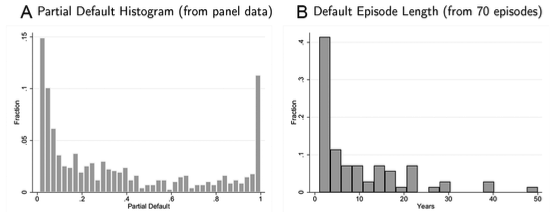
\includegraphics[width=0.7\textwidth]{../outputs/fig_2.png}
\caption{Partial default and default episode length.}
\end{figure}


\end{frame}

\begin{frame}{Empirics}

\begin{figure}
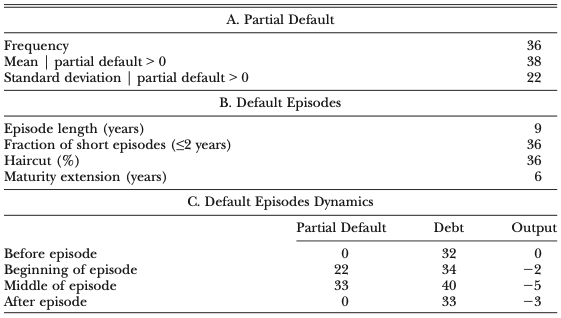
\includegraphics[width=0.7\textwidth]{../outputs/tab_1.png}
\caption{Partial default and default episodes in percentages.}
\end{figure}

    
\end{frame}

\begin{frame}{Empirics}

\begin{figure}
    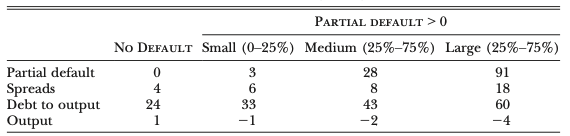
\includegraphics[width=0.7\textwidth]{../outputs/tab_2.png}
    \caption{Comovements.}
\end{figure}
 
\begin{itemize}
    \item Partial default is common,
    \item Higher partial default \(\leftrightarrow\) Higher spreads, higher debts, more depressed output,
    \item Hump-shape of the debt-to-output ratio, no reduction in debt.
\end{itemize}

\end{frame}

\section{Model}

\begin{frame}{Setting}

Consider a small open economy with:
\begin{itemize}
    \item A stream of stochastic endowments,
    \item A sovereign who:
    \begin{itemize}
        \item Borrows in long-term bonds,
        \item Chooses to partially default on the debt due.
    \end{itemize}
\end{itemize} 

\end{frame}

\begin{frame}{The sovereign's problem}

Let:
\smallbreak
\(z_t\) a stochastic endowment that follows a Markov process (transition probability: \(\pi(z_{t+1},z_t)\)),
\smallbreak    
\(E \Bigl\{ \sum_{t=0}^{+\infty} \beta^t u(c_t)\Bigr\}\) the objective function of the sovereign,
\smallbreak    
\(c_t=y_t-a_t(1-d_t)+q(a_{t+1},d_t,z_t)b_t\) the budget of the sovereign,
\smallbreak    
\(y_{t+1}=z_{t+1}\Psi(d_t,z_{t+1})\leq z_{t+1}\) the "production function" of income, with \(\Psi\) decreasing and concave in \(d_t\) and \(\Psi(0, z_{t+1}=1)\) (default carries a resource cost).
\bigbreak
Recall the accounting law of motion:
\[
  a_t
  = \delta a_t
  + (R-\delta)\kappa d_t a_t
  + b_t
  \]
Each period, the sovereign chooses \(\{d_t;b_t\}\) facing \(\{q_t;z_t\}\).

\end{frame}

\begin{frame}{The lenders' model}

    \begin{itemize}
        \item Purchase sovereign bonds by issuing securities at the risk-free world gross interest rate R.
        \item The value of 1 unit of existing debt today is equal to the discounted stream of payments, which is:
        \begin{itemize}
            \item The amount paid today (partially defaulted or not),
            \item The expected discounted continuation value,
        \end{itemize} 
        \item Free entry in the market drives profit to 0 and specifies \(q(a_{t+1},d_t,z_t)\),
        \item Partial default:
        \begin{itemize}
            \item Reduces the value held by lenders today,
        \item Increases the value held by lenders tomorrow,
        \item Affects the value lent by lenders tomorrow through its effect on output.
        \end{itemize}
    \end{itemize}

\end{frame}

\begin{frame}{Equilibrium in recursive terms}

The recursive Markov equilibrium consists in:
    \begin{itemize}
        \item The borrower's decision rules for:
        \begin{itemize}
            \item Borrowing \(b(a,y,z)\),
            \item Partial default \(d(a,y,z)\),
            \item Consumption \(c(a,y,z)\),
        \end{itemize} 
        Which induce debt due \(a'(a,y,z)\),
        \item The value of existing debt \(H(a,y,z)\),
        \item The bond price function \(q(a',d,z)\),  
    \end{itemize}
Such that:
\begin{itemize}
    \item Taking \(q(a',d,z)\) as given, the borrower's decision rule holds,
    \item Taking \(b(a,y,z)\), \(d(a,y,z)\), \(c(a,y,z)\) as given, the lenders' decision rule holds,
    \item \(q(a',d,z)\) yields zero profit. 
\end{itemize}    
\end{frame}

\begin{frame}{Teachings from the optimality conditions for the sovereign}
Debt and borrowing are capped diffently.
\bigbreak
FOC with respect to \(b\):
\begin{itemize}
    \item 1 extra unit of \(b\) increases consumption by \(q\) but reduces the price of debt (raising the raising the debt due) by \(q_{a'}\),
    \item This marginal gain from borrowing equals the marginal cost, which is the discounted expected value of increasing the debt burden.
\end{itemize}
Resources raised with borrowing are shaped by a laffer. curve\\

\bigbreak
FOC with respect to \(d\):
\begin{itemize}
    \item 1 extra unit of \(d\) increases consumption by \(a\) but reduces the price of debt (due to increasing future debt obligations and decreasing future resources) by \((q_{a'}(R-\delta)\kappa a + q_d)b\).
\end{itemize}
Resources raised with borrowing are not shaped by a laffer curve but have upper bound \(a\).

\end{frame}

\begin{frame}{Teachings from the optimality conditions for the sovereign}

The combination of both yields, for interior solutions (partial default), the portfolio condition:
\(R^b=R^d=\frac{u_c}{\beta E[u'_c]}\) (the expected return of marginal utility of consumption)\\
\bigbreak
For corner solutions (no partial default):
\(R^b<R^d\)
\bigbreak
In case of partial default, the next period sees \(R^d<R^b\) and, by virtue of the portfolio condition, the sovereign is incentivized to exit default

\bigbreak
Borrowing is an attractive way to smooth consumption when:
\begin{itemize}
    \item The price of new debt is high,
    \item The price of new debt decreases little marginally.
\end{itemize}
\bigbreak
Partial default is an attractive way to smooth consumption when:
\begin{itemize}
    \item The price of new debt is low,
    \item The price of new debt decreases a lot marginally.
\end{itemize}

\end{frame}

\begin{frame}{Teachings from the zero profit condition and the decision rule}

This specifies:
\begin{itemize}
    \item \(q_{a'}\):
    \begin{itemize}
        \item Negative effect from the higher likelyhood of a loss from not paying,
        \item The diluted continuation effect (continuation amount diluted because of the future borrowing and defaults).
    \end{itemize}
    \item \(q_{d'}\)
    \begin{itemize}
        \item Negative effect from the output cost of default,
        \item The diluted continuation effect (continuation amount diluted because of the future borrowing and defaults caused by the output decrease).
    \end{itemize}
\end{itemize}

\end{frame}

\section{Quantitative results}

\begin{frame}{Model calibration}

Set:
\smallbreak
\(u(c)=\frac{c^{1-\sigma}}{1-\sigma}\),
\smallbreak
\(log(z)\) follows an 11-state approximation of an autoregressive process,
\smallbreak
\(\Psi(z',d)=(1-\phi_0 d^\gamma)(1-\hat{\phi}_1(z'-z*))\) with \(\phi_0>0\), \(\gamma>1\), \(\hat{\phi}_1=\phi_1\) if \(d>0\).
\bigbreak
Other parameters estimated by minimum distance (sum of the proportional square residuals of 11 moments), averaged across the 37 countries.
\bigbreak
Model simulated for 750,000 periods with the first 10\% discarded.
    
\end{frame}

\begin{frame}{Simulation}
\begin{figure}
    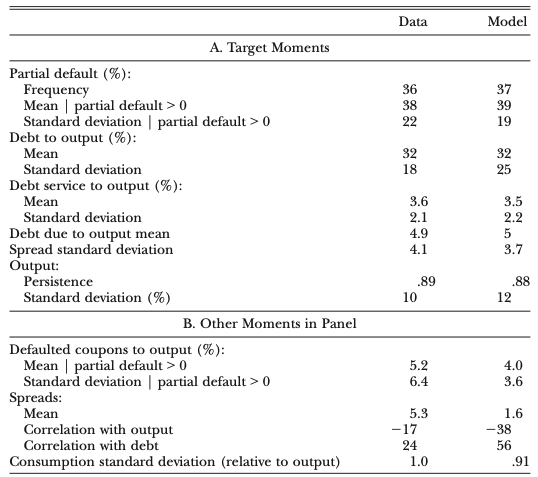
\includegraphics[width=0.7\textwidth]{../outputs/tab_4.png}
    \caption{Moments in model and data.}
\end{figure}
\end{frame}

\begin{frame}{Decision rules to enter partial default}
    \begin{figure}
        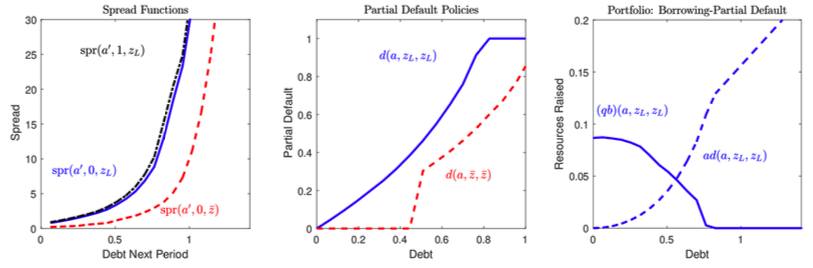
\includegraphics[width=1\textwidth]{../outputs/fig_3.png}
        \caption{Spreands, partial default, and portfolio.}
    \end{figure}
    \end{frame}

\begin{frame}{Bins for quantitative implications}
        \begin{figure}
            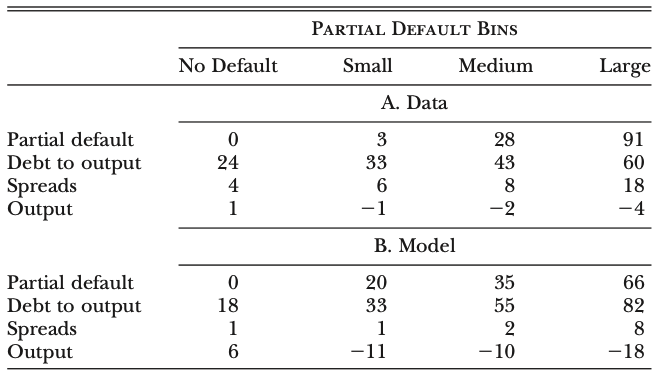
\includegraphics[width=0.7\textwidth]{../outputs/tab_5.png}
            \caption{Partial default, spreads, debt, and output.}
        \end{figure}
\end{frame}

\begin{frame}{Partial default episodes: length, haircuts, muaturity extensions}
    \begin{figure}
        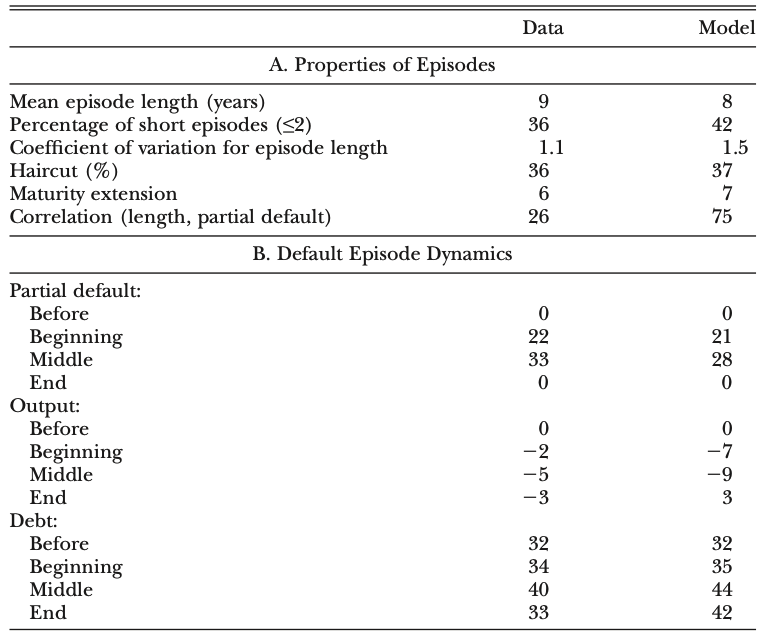
\includegraphics[width=0.7\textwidth]{../outputs/tab_6.png}
        \caption{Default episode properties.}
    \end{figure}
\end{frame}

\begin{frame}{Partial default episodes: dynamics}
    \begin{figure}
        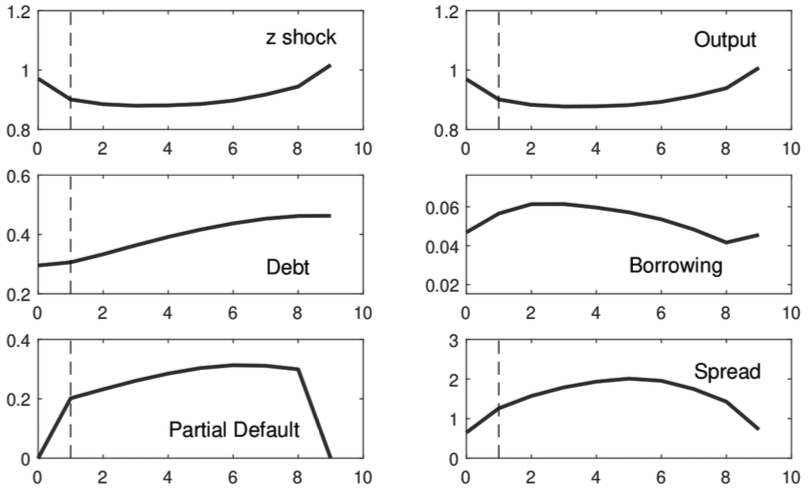
\includegraphics[width=0.7\textwidth]{../outputs/fig_4.png}
        \caption{Default episode properties.}
    \end{figure}
\end{frame}

\section{Conclusion}

\end{document}
% ||||||||||||||||||||||||||||||||||||||||||||||||||||||||||||||||||||
% ||||||||||||||||||||||||||||||||||||||||||||||||||||||||||||||||||||
% ||||||||||||||||||||||||||||||||||||||||||||||||||||||||||||||||||||